\let\negmedspace\undefined
\let\negthickspace\undefined
\documentclass[journal,12pt,onecolumn]{IEEEtran}
\usepackage{cite}
\usepackage{amsmath,amssymb,amsfonts,amsthm}
\usepackage{algorithmic}
\usepackage{graphicx}
\usepackage{textcomp}
\usepackage{xcolor}
\usepackage{txfonts}
\usepackage{listings}
\usepackage{enumitem}
\usepackage{mathtools}
\usepackage{gensymb}
\usepackage{comment}
\usepackage{caption}
\usepackage[breaklinks=true]{hyperref}
\usepackage{tkz-euclide} 
\usepackage{listings}

\usepackage{gvv}                                        
%\def\inputGnumericTable{}                                 
\usepackage[latin1]{inputenc}     
\usepackage{xparse}
\usepackage{color}                                            
\usepackage{array}                                            
\usepackage{longtable}                                       
\usepackage{calc}                                             
\usepackage{multirow}
\usepackage{multicol}
\usepackage{hhline}                                           
\usepackage{ifthen}                                           
\usepackage{lscape}
\usepackage{tabularx}
\usepackage{array}
\usepackage{float}
%\newtheorem{theorem}{Theorem}[section]
%\newtheorem{theorem}{Theorem}[section]
%\newtheorem{problem}{Problem}
%\newtheorem{proposition}{Proposition}[section]
%\newtheorem{lemma}{Lemma}[section]
%\newtheorem{corollary}[theorem]{Corollary}
%\newtheorem{example}{Example}[section]
%\newtheorem{definition}[problem]{Definition}

\begin{document}

\title{5.13.104}
\author{AI25BTECH11035 - SUJAL RAJANI}
% \maketitle
% \newpage
% \bigskip
%\begin{document}
{\let\newpage\relax\maketitle}
%\renewcommand{\thefigure}{\theenumi}
%\renewcommand{\thetable}{\theenumi}
% \newpage
% \bigskip
\textbf{QUESTION}
\\
Let $\vec{R}^2$ denote the Euclidean space . Let S={($a,b,c$):$a,b,c$$\epsilon$$\vec{R}$,$ax^2+2bxy+cy^2>0$$\forall(x,y)\epsilon\vec{R}^2-{(0,0)}$}.Then which of the following statement is (are) TRUE ?
\\
  (a) (2,$\frac{7}{2}$,6)$\epsilon$S
  \\
  \\
  (b) IF (3,b,$\frac{1}{12}$)$\epsilon$S,then $|2b|<1 $.
  \\
  \\
  (c)For any given ($a,b,c$)$\epsilon$S,the system of linear equations 
  \begin{align*}
      ax+by=1
      \\
      bx+cy=-1
  \end{align*}
  has a unique solution .
  \\
  (d) For any given ($a,b,c$)$\epsilon$S, the system of linear equations 
  \begin{align*}
      (a+1)x+by=0
      \\
      bx+(c+1)y=0
  \end{align*}
  has a unique solution .
  \\
\textbf{solution}
\\
as mentioned in the question :
\\
\begin{align*}
    ax^2+2bxy+cy^2>0\forall(x,y)\epsilon\vec{R}^2-{(0,0)}
\end{align*}
let Q be a matric :
\begin{align*}
    \vec{Q}=\myvec{a&b\\b&c}
\end{align*}
then:
\begin{align*}
    ax^2+2bxy+cy^2=\myvec{x&y}\myvec{a&b\\b&c}\myvec{x\\y}
\end{align*}
for this to happen :
\\
\begin{align*}
    a>0,c>0,||\vec{Q}||=ac-b^2>0 
\end{align*}
So,S={(a,b,c):$a>0$,$c>0$,$ac-b^2>0$}
option (a):
\\
$a=2>0$,c=6,b=$\dfrac{7}{2}$
\\
\begin{align*}
    ac-b^2=12-(\dfrac{7}{2})^2=-\dfrac{1}{4}<0
\end{align*}
option a is not correct .
\\
option b is correct :
\\
\begin{align*}
    a=3>0,ac-b^2=\dfrac{1}{4}-b^2>0,|2b|<1
\end{align*}
option b  is correct .
\\
option c :
\\
\begin{align*}
    ax+by=1,bx+cy=-1.
    \\
    \myvec{a&b\\b&c}\vec{x}=\myvec{1\\-1}
\end{align*}
for the solution to be unique:
\\
\begin{align*}
    ||\vec{Q}||=ac-b^2\neq0.
\end{align*}
from the definition os S,$ac-b^2>0$.
\\
option c is correct .
\\
option d is not correct 
\\
\begin{align*}
    (a+1)x+by=0,bx+(c+1)y=0.
\end{align*}
this type of homogeneous equation either have one solution or infinite solution .
\\
in case of one solution the solution is (0,0) which we do not get for any $$(a,b,c)\epsilon S$$.
        \begin{figure}[H]
    \centering
    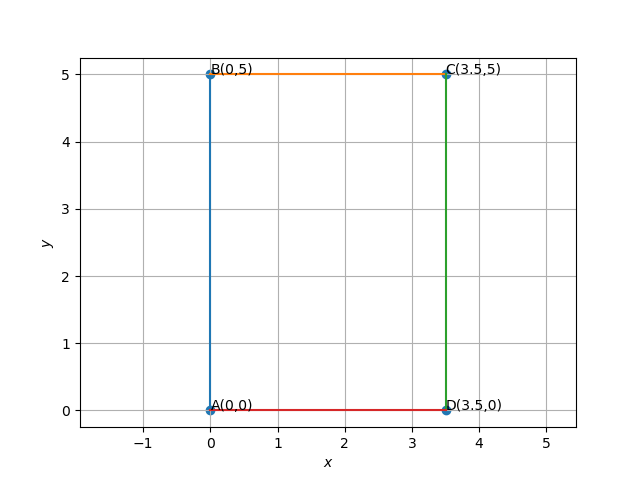
\includegraphics[width = 0.7\columnwidth]{../figs/img.png}
    \caption*{}
    \label{figs}
\end{figure}

\end{document}